\documentclass[11pt,letterpaper]{article}
\usepackage[margin=0.82in,headheight=15pt]{geometry}
\usepackage[T1]{fontenc}
\usepackage{lmodern,amsmath,amssymb,amsthm,mathtools,booktabs,array,graphicx}
\usepackage{xcolor,microtype,enumitem,fancyhdr}
\definecolor{navy}{HTML}{18384E}
\definecolor{teal}{HTML}{137F8C}
\definecolor{pale}{HTML}{EDF4F6}
\usepackage[colorlinks=true,linkcolor=navy,urlcolor=teal,citecolor=navy]{hyperref}
\hypersetup{pdftitle={Exact Internal Mode Sums for the Scalar Sector and Higgs-Induced Neutral Kinetics},pdfauthor={Prepared for Christopher Michael Baird with OpenAI Codex}}
\pagestyle{fancy}\fancyhf{}
\fancyhead[L]{\small\color{navy} MQGT--SCF / EXACT INTERNAL MODE SUMS}
\fancyhead[R]{\small 22 October 2026}
\fancyfoot[L]{\small Conditional spectral-action calculation}
\fancyfoot[R]{\small\thepage}
\setlength{\parindent}{0pt}\setlength{\parskip}{5pt}
\setlist{nosep,leftmargin=1.5em}\emergencystretch=2em
\DeclareMathOperator{\Tr}{Tr}\DeclareMathOperator{\diag}{diag}
\DeclareMathOperator{\tr}{tr}\DeclareMathOperator{\spec}{spec}
\newcommand{\dd}{\mathrm d}\newcommand{\Lam}{\Lambda}
\newcommand{\M}{\mathcal M}\newcommand{\B}{\mathcal B}
\newcommand{\HH}{\mathcal H}\newcommand{\kk}{\mathsf K}
\newcommand{\mm}{\mathsf M}
\newtheorem{proposition}{Proposition}
\newcommand{\ScalarTable}{\begin{tabular}{@{}lrrr@{}}\toprule
Coefficient & Local $a_2$--$a_4$ & Exact $f_-$ & $f_+-f_-$\\\midrule
$A_2$ & $-2.717741\times10^{-3}$ & $-3.247173902\times10^{-3}$ & $6.30042\times10^{-11}$\\
$G$ & $3.647588\times10^{-3}$ & $3.686749960\times10^{-3}$ & $1.89623\times10^{-9}$\\
$A_4$ & $1.935106\times10^{-4}$ & $1.696734060\times10^{-4}$ & $1.19954\times10^{-10}$\\
$C_0$ & $1.935106\times10^{-4}$ & $1.309313122\times10^{-4}$ & $8.65952\times10^{-11}$\\
$C_1$ & $1.935106\times10^{-4}$ & $2.084154998\times10^{-4}$ & $1.53313\times10^{-10}$\\
\bottomrule\end{tabular}}
\newcommand{\DownMatrix}{\begin{pmatrix}-0.02033237 & 0.00102316 & 0.06042393\\0.00102316 & -0.02103440 & 0.00393865\\0.06042393 & 0.00393865 & -0.23290731\end{pmatrix}}
\newcommand{\DownPhoton}{-0.03932044965}
\newcommand{\DownPhotonDelta}{-1.16663\times10^{-9}}
\newcommand{\UpMatrix}{\begin{pmatrix}-0.01524928 & -0.00288123 & -0.04531795\\-0.00288123 & -0.01672674 & -0.01800302\\-0.04531795 & -0.01800302 & -0.17468048\end{pmatrix}}
\newcommand{\UpPhoton}{-0.03773847661}
\newcommand{\UpPhotonDelta}{-2.54750\times10^{-9}}
\newcommand{\FixtureK}{\begin{pmatrix}0.199244396 & -0.000008263 & 0.000313358\\-0.000008263 & 0.200128772 & -0.000075598\\0.000313358 & -0.000075598 & 1.839750172\end{pmatrix}}
\newcommand{\FixtureMass}{\begin{pmatrix}2.1787216 & -2.1787216 & -1.5297173\\-2.1787216 & 2.1787216 & 1.5297173\\-1.5297173 & 1.5297173 & 8.7113578\end{pmatrix}}

\begin{document}
\thispagestyle{plain}
{\small\bfseries\color{teal} BAIRD / ZORAASI RESEARCH CONTINUATION}\par
{\LARGE\bfseries\color{navy} Exact internal mode sums for the scalar sector and Higgs-induced neutral kinetics}\par
{\large From the specified microscopic operator to finite-radius scalar coefficients and the photon residue}\par
\textbf{Prepared for Christopher Michael Baird with OpenAI Codex}\hfill 22 October 2026

\colorbox{pale}{\parbox{\dimexpr\linewidth-2\fboxsep\relax}{\textbf{Result.} The microscopic scalar insertion and the torsion-free geometric weak lift inherited from the preceding notes determine convergent internal-mode formulas for the scalar quadratic, wave-function and quartic coefficients, and for the full transverse neutral kinetic response. At the published common radius, the canonical quadratic mass parameter is $m_H^2/\Lam^2=-1.76153736$ for $f_-$, rather than the local value $-1.49015750$. The two mixed quartics split: $C_0=1.30931312\times10^{-4}$ and $C_1=2.08415500\times10^{-4}$. The neutral kinetic matrix acquires nonzero Higgs-dependent diagonal and mixing terms; the photon generator remains $Q=J_3+Y/2$ and its residue is still $(N^TKN)^{-1}$, $N=(1,1,0)^T$. The exact coefficients distinguish the inherited profile pair. All results are classical, conditional on the specified operator and background family. The measured fine-structure constant is not derived.}}

\section{Question, inputs, and scope of exactness}

The scalar/anomaly continuation \cite{scalar} fixed a Hermitian Higgs-dependent Dirac operator but used a six-dimensional local $a_2$--$a_4$ approximation for its scalar sector. Its gauge and radius coefficients used exact internal mode sums. This note removes that local approximation for the coefficients computed here. It also evaluates the Higgs-induced neutral kinetic shifts that were previously left as $\delta K$.

The common-vacuum pair is the unchanged 95-digit input from commit \texttt{3a8a1b0}; the scalar continuation is pinned at \texttt{7cfd341}. The supplied twelve-page geometric weak-response note \cite{weak} fixes the full off-product operator, including the spin-connection curvature vertex. Its PDF hash and the source hashes are recorded in \texttt{provenance.json}. We now \emph{recompute} the unbroken weak coefficient, rather than treating its printed value as the calculation's input.

Here ``exact'' means an internal spectral representation without a local expansion in $1/R$, where $R=\Lam r$. Numerical values come from finite angular cutoffs with convergence and independent-method checks. The scalar potential is expanded through fourth order in the lowest scalar harmonics, its kinetic coefficient through two external derivatives at zero scalar background, and the displayed neutral kinetic shifts through second order in aligned scalar amplitudes. A direct finite-background example is also supplied. These are not all-field or quantum effective-action results. The radius is held fixed; a new coupled vacuum is not asserted.

\section{Operator and monopole-harmonic realization}

The inherited action and profiles are
\begin{equation}
 S_{\rm sp}=\frac{\kappa}{2}\Tr_{\rm Dirac}f(D_6^2/\Lam^2),\qquad
 f(z)=\sum_{a\in\mathcal A}w_a e^{-az},\qquad w_a>0,\quad\sum_aw_a=1.
 \label{eq:action}
\end{equation}
A symbol $a$ below denotes one positive rate; all displayed physical kernels are its $w_a$-weighted sums. The fermion content, four copied blocks, colour weights and opposite six-dimensional chirality assignment are inherited, including their qualifications. The $n=2$ sectors are $Q,L$ and the $n=1$ sectors are $d,u,e$. The $n=0$ spectator has no Higgs coupling.

Write $\Gamma=\sigma_3$ on the internal spinor, and set
\begin{equation}
 \Phi_i=\frac1r\sum_{m=\pm1/2}H_{i,m}Y_{1/2,m},\quad
 h_i=\frac{H_i}{\Lam R},\quad y_{6,i}=\frac{\widehat y_i}{\Lam},\quad
 \frac{\M}{\Lam}=\begin{pmatrix}0&\widehat y_i h_iY\\
 \widehat y_i\overline h_iY^\dagger&0\end{pmatrix}.
 \label{eq:units}
\end{equation}
The internal dimensionless Hermitian operator is
\begin{equation}
 \B(h)=\frac{D_n}{R}+\Gamma\frac{\M(h)}{\Lam},\qquad
 D_6/\Lam=\gamma^\mu p_\mu+\gamma_5\B(h)
 \quad\hbox{at zero external gauge field}.\label{eq:B}
\end{equation}
The phase convention is chosen so that the massive entries of $D_n$ are real and positive. In internal chirality $\tau=\pm1$, the basis consists of spin-weighted monopole harmonics with
\begin{equation}
 s_\tau=\frac{n-\tau}{2},\quad j=|s_\tau|,|s_\tau|+1,\ldots,\quad
 E_j=j(j+1)-\frac{n^2-1}{4},\quad
 (D_n)_{+,j,m;-,j,m}=\sqrt{E_j}.
 \label{eq:monopole}
\end{equation}
Thus $\Tr_{\rm int}e^{-uD_n^2}=n+2\sum_{\ell\ge1}(2\ell+n)e^{-u\ell(\ell+n)}$ for $n\ge0$, with the $n=0$ zero term absent. This reproduces exactly twice the inherited $\widehat h_n$ convention. Monopole-spinor representations and zero modes follow the framework of \cite{Jante}; our explicit scalar multiplication matrices are specified next.

For a charge-$+1$ scalar harmonic of spin weight $1/2$, its matrix from the $n=1$ to the $n=2$ spinor space is
\begin{multline}
 U^{(m_H)}_{J,m+m_H;j,m;\tau}
 =\sqrt{\frac{2(2j+1)}{4\pi(2J+1)}}\,
 \langle j,m;\tfrac12,m_H|J,m+m_H\rangle\\
 {}
 \times\langle j,-s_\tau;\tfrac12,-\tfrac12|J,-s_\tau-\tfrac12\rangle,
 \qquad J=j\pm\tfrac12 .\label{eq:U}
\end{multline}
It vanishes unless the target exists. The second Clebsch--Gordan coefficient fixes the spin-weight convention, including relative chiral phases. At the zero modes, the overlap is $1/\sqrt{4\pi}$. The implementation checks 106 entries of \eqref{eq:U} against independent sphere quadrature of factorial-sum Wigner functions.

For neutral aligned doublets, the down map uses $m_H=-1/2$ and the conjugate-up map uses $m_H=+1/2$. Then $m_Q=m_d-1/2=m_u+1/2$, and $m+q_Y$ is constant within each mixed block. In the quark sector $q_Y=(1/6,-1/3,2/3)$; in the lepton sector it is $(-1/2,-1)$. These facts give an efficient block decomposition and enforce $[\B,Q]=0$ at nonzero neutral background.

\section{Exact scalar kernels}

\subsection{Potential normalization and two-insertion coefficients}

External momentum integration and the four-component external spin trace give the potential density
\begin{equation}
 \frac{V(h)-V(0)}{\kappa\Lam^4}
 =\frac1{8\pi^2}\sum_a\frac{w_a}{a^2}
 \Tr_{\rm int}\left(e^{-a\B(h)^2}-e^{-a\B(0)^2}\right).
 \label{eq:potential}
\end{equation}
The internal trace includes flavours and colours when present. For the universal one-link coefficients below it contains just one $n=2$ and one $n=1$ species. No new isometry representation multiplicity is inserted.

Let $\B(h)=B+hS$ along one real harmonic, $E=B^2$, $A=\{B,S\}$ and $Z=S^2$. In an eigenbasis $B_{ij}=b_i\delta_{ij}$, put $e_i=b_i^2$ and
\begin{align}
 I_0^{ij}(a)&=\int_0^1e^{-a[se_i+(1-s)e_j]}\dd s,\\
 I_u^{ij}(a)&=\int_0^1s(1-s)e^{-a[se_i+(1-s)e_j]}\dd s,\qquad
 I_o^{ij}=a(e_i-e_j)I_u^{ij}.\label{eq:moments}
\end{align}
The last equality follows by integrating the derivative of $s(1-s)$; $I_o$ is the same integral with weight $1-2s$. These divided-difference kernels retain transitions between unequal internal energies.

Cyclicity of the Duhamel expansion \cite{Iochum} gives
\begin{align}
 A_2(a,R)&=\frac1{8\pi^2}\left[-\frac1a\Tr(Z e^{-aE})+
       \frac12\sum_{ij}I_0^{ij}|A_{ij}|^2\right],\label{eq:A2}\\
 G(a,R)&=\frac1{8\pi^2}\sum_{ij}
       \left[I_0^{ij}|S_{ij}|^2-aI_u^{ij}|A_{ij}|^2\right].\label{eq:G}
\end{align}
The field convention is $V/(\kappa\Lam^4)=A_2h^2+A_4h^4+\cdots$ and $\mathcal L_{\rm kin}=\kappa\Lam^2(G/2)(\partial h)^2$ on this real slice. For a complex doublet, the coefficient of $|\partial h|^2$ is also $\kappa\Lam^2G/2$. Equation~\eqref{eq:G} follows from the scalar Fourier vertex: the linear insertion in $D_6^2$ is $\{B,S\}+q\gamma^1\gamma_5S$, and the shifted Gaussian contributes $e^{-as(1-s)q^2}$. It does not assume a local heat expansion.

\subsection{Quartic extraction without finite differences}

At a finite internal cutoff, form a five-by-five block upper-triangular matrix
\begin{equation}
 \HH=\begin{pmatrix}
 E&A&Z&0&0\\0&E&A&Z&0\\0&0&E&A&Z\\0&0&0&E&A\\0&0&0&0&E
 \end{pmatrix}.
 \label{eq:toeplitz}
\end{equation}
The block $(0,k)$ of $e^{-a\HH}$ is exactly $[h^k]e^{-a(E+hA+h^2Z)}$ for $k\le4$. Thus
\begin{equation}
 A_4(a,R)=\frac1{8\pi^2a^2}\tr\bigl(e^{-a\HH}\bigr)_{0,4}.
 \label{eq:A4}
\end{equation}
This is a finite-matrix identity; the spectral coefficient is its cutoff limit. It is checked by a separate Cauchy-contour evaluation of \eqref{eq:potential}, using eigenvalues of $B+hS$ at complex $h$. The latter does not use the block exponential.

All coefficient sums converge for positive $a$ and finite positive $R$. The scalar multiplication and the differentiated Yukawa insertion are bounded on the sphere; their angular matrices are banded. At each finite Taylor order a trace path visits only finitely separated angular levels. Polynomial angular factors are dominated by Gaussian spectral decay. This supports differentiation and summation at the orders used here. It is not a numerical interval certificate for the printed values; finite-boundary products and roundoff are tested by increasing the cutoff.

\subsection{Two-doublet invariant potential}

Define $D=h_d^\dagger h_d$, $U=h_u^\dagger h_u$ and $P=|h_d^Ti\sigma_2h_u|^2$. The exact quartic potential on the retained harmonics has the form
\begin{align}
 \frac{V}{\kappa\Lam^4}={}&N_bA_2\left[(3\widehat y_d^2+\widehat y_e^2)D+3\widehat y_u^2U\right]\nonumber\\
 &+N_bA_4\left[(3\widehat y_d^4+\widehat y_e^4)D^2+3\widehat y_u^4U^2\right]\nonumber\\
 &+3N_b\widehat y_d^2\widehat y_u^2(C_0DU+C_1P)+O(h^6),\label{eq:2HDM}\\
 \frac{\mathcal L_{\rm kin}}{\kappa\Lam^2}={}&\frac G2N_b\left[(3\widehat y_d^2+\widehat y_e^2)|D_\mu h_d|^2+
                  3\widehat y_u^2|D_\mu h_u|^2\right]+O(h^2|D h|^2).
 \label{eq:kinH}
\end{align}
Here and below the rate sum is implicit in $A_2,G,A_4,C_0,C_1$. Generation-diagonal real Yukawas are retained; complex phases are unnecessary for the CP-conserving fixtures.

To evaluate $C_0$, set the two maps into $Q$ to orthogonal scalar components, with equal real amplitudes $h$; if their quartic coefficient is $A_4^{\perp}$, then $C_0=A_4^{\perp}-2A_4$. If the two maps are parallel, a unitary rotation of the identical internal $n=1$ spaces replaces $h$ by $\sqrt2h$ in a single link, leaving one uncoupled space. Hence the exact identity
\begin{equation}
 C_0+C_1=2A_4.\label{eq:quarticidentity}
\end{equation}
This identity concerns the scalar potential at zero external gauge background, where the right-sector charge differences do not enter the operator. It does \emph{not} imply $C_0=C_1$. That stronger equality was a consequence of the local sphere integral in the predecessor.

\section{Scalar results at the common radius}

The inherited radius is $R_*=1.278472412043978650\ldots$, with $m_1=m_2=0.5535574693051822\ldots$. The local controls, in the field convention \eqref{eq:units}, are
\begin{equation}
 A_2^{\rm loc}=\frac{-2R^2m_2+5m_1/6}{16\pi^3},\quad
 G^{\rm loc}=\frac{R^2m_1}{8\pi^3},\quad
 A_4^{\rm loc}=C_0^{\rm loc}=C_1^{\rm loc}=\frac{R^2m_1}{48\pi^4}.
 \label{eq:local}
\end{equation}
The computed values are:
\begin{center}\footnotesize\ScalarTable\end{center}
The $f_+$ coefficient is the exact $f_-$ column plus the last column. More digits and all ten single-rate kernels are in \texttt{results.json}. Differences are formed from the weight difference applied to the single-rate kernels, avoiding subtraction of profile totals.

\begin{figure}[ht]
\centering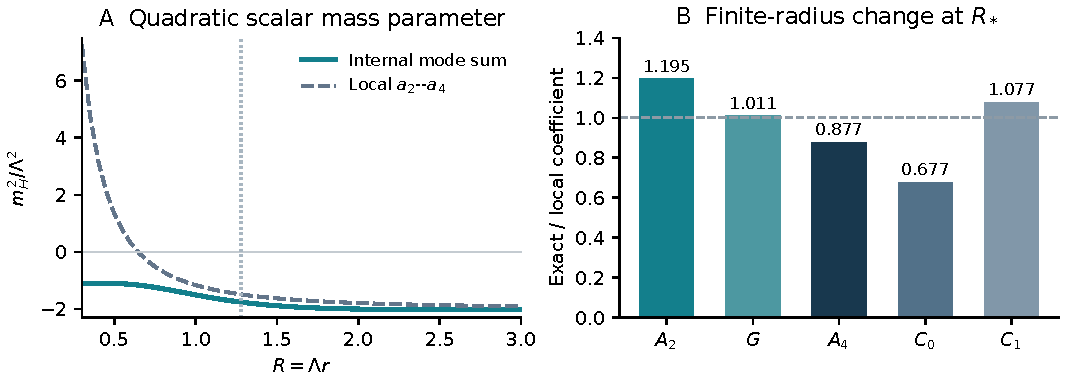
\includegraphics[width=\linewidth]{images/scalar_response.pdf}
\caption{Fixed-radius scalar calculation for $f_-$. Left: quadratic mass parameter from the internal mode sums compared with the local $a_2$--$a_4$ truncation; the dotted line marks $R_*$. This is a scan of coefficients, not a family of solved vacua or physical pole masses. Right: finite-radius changes in the five coefficients at $R_*$. The two mixed quartics no longer coincide.}
\end{figure}

Canonical normalization gives
\begin{equation}
 \frac{m_H^2}{\Lam^2}=\frac{2A_2}{G}
 =\begin{cases}-1.76153736315,&f_-,\\-1.76153642295,&f_+,
 \end{cases}
 \qquad \left(\frac{m_H^2}{\Lam^2}\right)_{\rm loc}=-1.49015750336.
 \label{eq:massresult}
\end{equation}
Here $m_H^2$ is the ratio of the zero-momentum quadratic coefficient to its two-derivative normalization, not a physical pole mass. Its magnitude is of order $\Lam^2$, so locating a pole would require the momentum-dependent kernel beyond this derivative expansion. Both doublets share the parameter because their multiplicities and Yukawa squares multiply $A_2$ and $G$ in the same way. The exact unbroken scalar wave-function factor is positive. For $N_b=4$ and unit $\widehat y_d,\widehat y_e,\widehat y_u$, the canonical quartics for $f_-$ are
\begin{equation}
 \kappa(\lambda_d,\lambda_u,\lambda_{DU},\lambda_P)
 =(3.12080346,\ 4.16107127,\ 2.40822001,\ 3.83338690).
\end{equation}
The positive alignment coefficient favours $P=0$, as before, but its magnitude and its relation to the other cross term change. These are expansion coefficients at zero scalar background. A minimum of the quartic polynomial is not a controlled global minimum of the untruncated spectral action.

\begin{proposition}[Small-radius zero-mode limit]
For fixed positive rates and a finite mixture, the one-link coefficients satisfy
\begin{equation}
 A_2\longrightarrow-\frac{m_1}{16\pi^3},\quad
 G\longrightarrow\frac{f(0)}{16\pi^3},\quad
 A_4\longrightarrow\frac{f(0)}{128\pi^4},\quad
 C_0\longrightarrow0,\quad C_1\longrightarrow\frac{f(0)}{64\pi^4},
 \quad(R\to0),\label{eq:smallR}
\end{equation}
and $m_H^2/\Lam^2\to-2m_1/f(0)$.
\end{proposition}
\begin{proof}
All nonzero internal Dirac eigenvalues grow as $1/R$. In the zero-mode subspace one scalar component couples one of the two $n=2$ zero modes to the $n=1$ zero mode, with eigenvalues $\pm h/\sqrt{4\pi}$; the other zero mode is unpaired. Its heat-trace change is $2(e^{-ah^2/(4\pi)}-1)$. Equations~\eqref{eq:potential} and \eqref{eq:G} give the first three limits. Orthogonal down and conjugate-up components couple independent zero-mode pairs, so their cross term vanishes. Equation~\eqref{eq:quarticidentity} gives the last limit. Bounded off-zero-mode insertions have vanishing contributions to these limits after the appropriate divided differences; the nonzero-mode gap diverges.
\end{proof}
The local positive small-$R$ mass term therefore cannot be extrapolated into the exact small-radius regime. The numerical scan in the bundle finds a negative exact mass throughout $0.3\le R\le3$ for this profile. It does not establish a global sign theorem at all radii.

\section{Complete neutral transverse response}

\subsection{Geometric vertex and definition of the coefficient}

Use neutral generators $T_a=(J_3,q_Y,x)$, labelled $(W,B,X)$. The inherited geometric operator contains the fixed spin-connection term \cite{weak,Baptista,Kaad}
\begin{equation}
 D_6=D_4^{\mathcal A}+\gamma_5\otimes(D_n/r+\Gamma\M)
       -\frac{ir}{8}F^W_{\mu\nu}\gamma^{\mu\nu}\gamma_5\otimes L,
 \qquad L=\sigma_2\sin\theta.
 \label{eq:fullD}
\end{equation}
Both ordered indices $\mu,\nu$ are summed. In the matrix convention of \eqref{eq:monopole}, $L=-\Gamma[D_n,C_\theta]$, where
\begin{align}
 (C_\theta)_{j,j;m}&=-\frac{s_\tau m}{j(j+1)},\\
 (C_\theta)_{j,j+1;m}&=
 \sqrt{\frac{((j+1)^2-m^2)((j+1)^2-s_\tau^2)}{(j+1)^2(2j+1)(2j+3)}}.
 \label{eq:C}
\end{align}
The $j=0$ diagonal is zero. These recurrence relations fix the geometric vertex independently of the scalar multiplication matrix.

At constant Higgs background, excite $\mathcal A_2^a(x_1)$ at momentum $q$. The quadratic response defines
\begin{equation}
 S^{(2)}=\int_q\mathcal A_2^a(-q)
       \bigl[M_{ab}^2+q^2K_{ab}+O(q^4/\Lam^2)\bigr]
       \mathcal A_2^b(q),\label{eq:operational}
\end{equation}
where this notation counts the paired Fourier modes once. Equivalently, it is the usual $\frac12\mathcal A(M^2+q^2K)\mathcal A$ convention integrated over all momenta. This operational transverse definition includes contributions from all covariant operators at this order. It must not be read as only the coefficient of $(H^\dagger H)F^2$ in an unspecified Wilson basis.

\subsection{Spectral formula in the broken background}

Diagonalize the full $\B(h)$, with eigenvalues $b_i$, not just $D_n$. Transform all insertions into that basis and define
\begin{equation}
 c=\frac R4,\quad L_W=L,\quad L_B=L_X=0,\quad
 C_a=[\B,T_a],\quad V_a=-T_a+c\{\B,L_a\}.
\end{equation}
For real aligned backgrounds the matrices can be chosen real, with $T_a,L_a,V_a$ symmetric and $C_a$ antisymmetric. Thus $(C_a)_{ij}=(b_i-b_j)(T_a)_{ij}$. All products within the sums below are entrywise at the same pair $i,j$; contact terms are ordinary matrix traces. The single-rate kernel is
\begin{align}
 \kk_{ab}(a,h)=\frac1{8\pi^2}\bigg\{\sum_{ij}\Big[&
 I_0^{ij}\left((V_a)_{ij}(V_b)_{ij}+\frac{4c^2}{a}(L_a)_{ij}(L_b)_{ij}\right)\nonumber\\
 &+cI_o^{ij}\left((C_a)_{ij}(L_b)_{ij}+(C_b)_{ij}(L_a)_{ij}\right)\nonumber\\
 &-I_u^{ij}\left(2(T_a)_{ij}(T_b)_{ij}+a(C_a)_{ij}(C_b)_{ij}\right)\Big]
 -\frac{2c^2}{a}\Tr(L_aL_b e^{-a\B^2})\bigg\}.\label{eq:Kmaster}
\end{align}
The corresponding zero-momentum mass kernel is
\begin{equation}
 \mm_{ab}(a,h)=\frac1{8\pi^2}\left\{\frac2a\left[
 \sum_{ij}I_0^{ij}(T_a)_{ij}(T_b)_{ij}-\Tr(T_aT_b e^{-a\B^2})\right]
 +\sum_{ij}I_0^{ij}(C_a)_{ij}(C_b)_{ij}\right\}.
 \label{eq:Mmaster}
\end{equation}
Rate and species sums give $K/\kappa=\sum_aw_a\kk$ and $M^2/(\kappa\Lam^2)=\sum_aw_a\mm$. The $n=0$ spectator contributes to unbroken $K$ but cancels in its Higgs-induced shift. A separately specified pure-$X$ Stueckelberg mass can be added to $M^2$; its microscopic value remains outside this calculation.

At $h=0$, $C_a=0$. For an external charge commuting with the operator and with $L_a=0$, \eqref{eq:Kmaster} reduces to $\Tr(T_a^2e^{-a\B^2})/(12\pi^2)$, recovering the inherited hypercharge normalization. For the geometric weak field it reduces to the complete four-term response of \cite[Eq.~(19)]{weak}, including its orbital, spin-potential, Pauli-square and Pauli-derivative terms. The computation reproduces
\begin{equation}
 \frac{K^{(0)}_-}{\kappa}=\diag(0.199544788403315,\ 0.200445639903623,\ 1.843191195308219).
\end{equation}
All unbroken off-diagonal entries cancel with the full content.

\section{Higgs-induced matrices and the photon residue}

\subsection{Leading shifts and normalization checks}

For $N_b=4$ and unit dimensionless Yukawas, at the inherited radius define
\begin{equation}
 \frac{K(h)}\kappa=\frac{K^{(0)}}\kappa+h_d^2D_d+h_u^2D_u+O(h^4).
 \label{eq:Ddef}
\end{equation}
The real $h_i$ are neutral component amplitudes in \eqref{eq:units}, not canonical vevs. For $f_-$ the full matrices are
\begin{align}
 D_d&=\DownMatrix,\label{eq:Dd}\\[3pt]
 D_u&=\UpMatrix.\label{eq:Du}
\end{align}
Both profiles, their matrix differences and the single-rate kernels are in the bundle. These coefficients were extracted by Cauchy differentiation of the analytic response, checked with a second contour and a real-background Richardson calculation. The complex extension uses a similarity eigenbasis and index-reversed products, never absolute squares of complex continuation data.

A useful check ties \eqref{eq:G} to \eqref{eq:Mmaster}. With $t_d=(-1/2,1/2,1)^T$ and $t_u=(-1/2,1/2,-1)^T$, one obtains
\begin{equation}
 \frac{M^2}{\kappa\Lam^2}=16G h_d^2t_dt_d^T+12G h_u^2t_ut_u^T+O(h^4).
 \label{eq:Ward}
\end{equation}
This agrees with the gauge masses derived directly from \eqref{eq:kinH}. In conventional canonical notation $\widehat H_i^0=\widehat v_i/\sqrt2$, the leading relation is $\widehat v_d^2=16\kappa\Lam^2G h_d^2$ and $\widehat v_u^2=12\kappa\Lam^2G h_u^2$. Thus equal bare $h_i$ between profiles is not precisely equal canonical vev.

\subsection{Massless generator and kinetic shift}

For the neutral background, $[\B,Q]=0$ with $Q=J_3+q_Y$; the exact mass kernel \eqref{eq:Mmaster} therefore annihilates $N=(1,1,0)^T$. The pure-$X$ Stueckelberg term does too. Where the other neutral directions are massive, the low-momentum transverse residue is
\begin{equation}
 \underset{p^2=0}{\operatorname{Res}}(p^2K+M^2)^{-1}
 =N(N^TKN)^{-1}N^T,\qquad e^{-2}=N^TKN.
\end{equation}
Consequently
\begin{align}
 \frac{e^{-2}_-}{\kappa}
 &=0.399990428306938\DownPhoton\,h_d^2\UpPhoton\,h_u^2+O(h^4),\label{eq:photon}\\
 \Delta\!\left(\frac{e^{-2}}\kappa\right)
 &=1.55190800181\times10^{-7}
   \DownPhotonDelta\,h_d^2\UpPhotonDelta\,h_u^2+O(h^4).
 \label{eq:deltaphoton}
\end{align}
The $X$ row drops out of this projection, while the $WB$ term is essential. The leading Higgs corrections to the pair difference are small at small $h$ and do not cancel the inherited unbroken difference. Equations~\eqref{eq:photon}--\eqref{eq:deltaphoton} compare a common prescribed radius and common bare amplitudes. They are not predictions for two self-consistent physical vacua.

\subsection{Finite-background example}

At $(h_d,h_u)=(0.10,0.08)$, evaluating the response directly rather than truncating \eqref{eq:Ddef} gives, for $f_-$,
\begin{align}
 K/\kappa&=\FixtureK,\\
 M^2/(\kappa\Lam^2)&=10^{-4}\FixtureMass
 \quad\hbox{before a Stueckelberg term}.
\end{align}
The kinetic matrix is positive definite and $M^2N=0$ to numerical precision. The photon value is $e^{-2}_-/\kappa=0.399356642050$, and the profile difference is $1.55162664\times10^{-7}$. The difference between this photon value and its $O(h^2)$ approximation is $9.44\times10^{-7}$, displaying the finite-field truncation error instead of treating the quadratic approximation as exact. This is an externally specified diagnostic background, not a solved vacuum.

\section{Local-order correction and radius matching data}

\subsection{A correction to the predecessor's kinetic-shift order counting}

The predecessor's A9 located the leading Higgs-induced shift at the six-dimensional $a_6$ field-strength terms. That statement is incomplete for a \emph{geometric} weak field. The scalar $a_4$ density already contains $(2/3)\mathcal R_6\tr\M^2$ \cite{Vass,scalar}, while the specified fibration has
\begin{equation}
 \mathcal R_6=\mathcal R_4+\frac2{r^2}
       -\frac{r^2}{4}\sin^2\theta\,F^W_{\mu\nu}F_W^{\mu\nu}
\end{equation}
in the Cartan direction at fixed radius. For one Yukawa link, $\tr\M^2=2\Lam^2h^2|Y|^2$ and $\int\sin^2\theta|Y|^2\dd\Omega=2/3$. Matching to $K_{WW}F_W^2/4$ gives the leading large-radius contribution
\begin{equation}
 [h^2]\frac{\delta K_{WW}^{(a_4)}}\kappa
 =-\frac{m_1R^4}{144\pi^3}\qquad\hbox{per one unit-Yukawa link}.
 \label{eq:a4correction}
\end{equation}
For a single exponential, the full-to-leading ratios at $R=2$, $4$ and $8$ are $1.40695$, $1.10703$ and $1.02719$, approaching the predicted leading term. Additional $a_6$ and higher terms remain. The finite-local-order equality for the inherited pair is unchanged, because $m_1$ and the other retained local moments agree. The exact finite-radius kernels are what lift that equality here.

\subsection{Weak response away from the inherited radius}

Reconstructing the geometric operator also supplies the derivative omitted from the predecessor scalar note:
\begin{equation}
 \left.\frac{\dd z_W}{\dd R}\right|_{R_*}
 =\begin{cases}0.406397405812,&f_-,\\0.406397190585,&f_+.
 \end{cases}
 \qquad
 \left.\frac{\dd z_Y}{\dd R}\right|_{R_*,f_-}=0.225141216662.
\end{equation}
These are derivatives of the unbroken exact kernels, evaluated with a fourth-order symmetric difference and a halved-step check. They complete an input to a future coupled-radius matching calculation. Substituting the old locally approximated vacuum shifts would mix schemes again, so that is not done here. The exact scalar coefficients and their radius dependence must enter the new stationarity problem consistently.

\section{Reproducibility, error scope, and physical interpretation}

The recorded run passes 126 checks. That count includes separate magnetic-block identities and is not a count of independent physical predictions. The main validation paths are:
\begin{center}\small
\begin{tabular}{@{}p{0.60\linewidth}r@{}}\toprule
Comparison & Largest reported difference\\\midrule
106 scalar-harmonic overlaps vs sphere quadrature & $7.30\times10^{-15}$\\
Scalar block exponential vs Cauchy contour & $2.38\times10^{-14}$\\
Neutral kernel vs full finite-$q$ external Clifford calculation & $2.56\times10^{-14}$\\
Scalar coefficients, cutoff 10 to 12 & $6.94\times10^{-18}$\\
Kinetic shift coefficients, cutoff 10 to 12 & $4.73\times10^{-14}$\\
Kinetic shifts, changed contour radius and point count & $2.56\times10^{-14}$\\
Kinetic Cauchy vs real-background Richardson & $5.08\times10^{-11}$\\\bottomrule
\end{tabular}
\end{center}
All entries refer to their defined numerical objects, not a common error norm on physical observables. The cutoff comparisons include each rate and each matrix entry. The two contour choices are radius $0.2$ with 16 points and radius $0.3$ with 24 points. No interval rounding enclosure, universal tail certificate, or external peer review is claimed. The 95-digit source input is preserved, but new numerical results use binary64/complex128 arithmetic; printed precision follows the independent checks, not the input's digit count.

The package contains the note, complete LaTeX source, unchanged inputs, per-rate numerical kernels, both profile evaluations, convergence records, the independent checks, assumptions, provenance, licence and checksums. Run \texttt{python run\_all.py} with NumPy and SciPy to regenerate the numerical results; \texttt{python build\_figures.py} regenerates the figure and tables with Matplotlib. The existing source compiles with \texttt{pdflatex main.tex}, twice. Checksums should be verified before rerunning archived files, because the scripts overwrite their result files.

The outcome is a completion of the previously unevaluated \emph{classical internal spectral coefficients} for the stated operator, at the stated field and momentum orders. It does not establish a unique microscopic completion, the six-dimensional anomaly polynomial, the axion reduction, a new coupled scalar/radius vacuum, or full compactification stability. Higher bosonic fields have not been integrated out. The heat-kernel parameter here belongs to the classical spectral action; this calculation is not a quantum loop integral.

For quantum matching one can now use the computed $K(h,R)$, $M^2(h,R)$ and scalar normalization as tree-level boundary data once the physical background is fixed. A consistent heavy spectrum, renormalization prescription, threshold corrections and running are still needed. The parameter $\kappa$ and the physical profile require independent specification. The conditional relation
\begin{equation}
 \alpha^{-1}_{\rm tree}=4\pi\kappa\,N^T\bigl(K(h,R)/\kappa\bigr)N
\end{equation}
is therefore not a prediction of the measured fine-structure constant. No measured coupling has been fitted or inserted.

\appendix
\section{External-momentum derivation of the neutral kernel}

This appendix fixes the momentum and seagull conventions in \eqref{eq:Kmaster}. Set $\Lam=1$ temporarily, take momentum transfer $q$ along direction 1 and a transverse potential in direction 2. With $\gamma^{12}=\gamma^1\gamma^2$, the first-order Dirac vertex is
\begin{equation}
 \delta D_a(q)=-\gamma^2T_a+cq\gamma^{12}\gamma_5L_a,
 \qquad \delta D_a(-q)=\delta D_a(q)^\dagger.
\end{equation}
Writing $D_0(p)=\gamma\cdot p+\gamma_5\B$, the linear insertion into $D^2$ is $D_0(p+q)\delta D(q)+\delta D(q)D_0(p)$, namely
\begin{align}
 H_{1,a}(p+q,p)={}&-2p_2T_a+\gamma^2\gamma_5C_a
       +q\gamma^{12}V_a\nonumber\\
 &+2cq(p_1\gamma^2\gamma_5-p_2\gamma^1\gamma_5)L_a
       +cq^2\gamma^2\gamma_5L_a.\label{eq:H1}
\end{align}
The quadratic insertion is the sum of the two ordered products of $\delta D(q)$ and $\delta D(-q)$. Omitting it would give an incorrect contact term and an incorrect mass identity.

In the two-insertion heat trace, shift $p_1=k_1-sq$. The Gaussian contributes $e^{-as(1-s)q^2}$ and $\langle k_1^2\rangle=\langle k_2^2\rangle=1/(2a)$. Orthogonality of the four external Clifford structures in \eqref{eq:H1} gives, for one real generator combination and each internal pair,
\begin{multline}
 \frac14\langle\tr_4 H_1^\dagger H_1\rangle
 =\frac2a T_{ij}^2+C_{ij}^2\\
 {}+q^2\left[V_{ij}^2+\frac{4c^2}{a}L_{ij}^2
              +2c(1-2s)C_{ij}L_{ij}\right]+O(q^4).
\end{multline}
Expanding the shifted Gaussian supplies the negative $I_u$ terms. The seagull supplies $-2c^2\Tr(L^2e^{-a\B^2})/a$ to the kinetic coefficient. Combining both Fourier orientations, the factor $\kappa/2$ and the external Gaussian $(4\pi a)^{-2}$ gives \eqref{eq:Kmaster}; polarization gives the mixed entries. The zero-momentum term gives \eqref{eq:Mmaster}.

The independent check constructs the full external-Clifford matrices before taking any trace, integrates their Gaussian moments and the insertion parameter, and extracts the coefficient from nonzero $q$. It tests a noncommuting three-state internal example with both $T$ and $L$ nontrivial. This checks the commutator and mixed Pauli terms, beyond the commuting unbroken limit.

\section{Stable heat moments and numerical coefficient extraction}

For real energies, let $d=a(e_i-e_j)$, $t=|d|$ and $z=a\min(e_i,e_j)$. Then
\begin{equation}
 I_0=e^{-z}\frac{1-e^{-t}}{t},\qquad
 I_u=e^{-z}\frac{t-2+(t+2)e^{-t}}{t^3},\qquad I_o=dI_u.
\end{equation}
At coincident energies these become $e^{-ae_i}$, $e^{-ae_i}/6$ and zero. The code uses convergent Taylor series near coincidence and \texttt{expm1} away from it. An independent Gauss--Legendre quadrature checks these formulas.

For the kinetic $h^2$ coefficient, holomorphic continuation provides
\begin{equation}
 [h^2]K(h)=\frac1{2\pi\rho^2}\int_0^{2\pi}
       K(\rho e^{i\theta})e^{-2i\theta}\dd\theta.
\end{equation}
The finite-dimensional response is analytic, even in a single real scalar direction, and admits this continuation. The code uses general eigenvectors and their inverse, retaining matrix-product contractions; it does not extend the real formula by taking complex absolute values. A second contour and direct real-background extrapolation quantify discretization and roundoff sensitivity. Internal cutoffs are imposed on full multiplets and then increased; no physical claim is attached to the cutoff itself.

\clearpage
\begin{thebibliography}{9}\small
\bibitem{scalar} Baird / ZoraASI Research Continuation, \emph{A Microscopic Scalar and Anomaly-Complete Sector for the Shared Spectral Action}, 22 October 2026. \href{https://github.com/Cbaird26/mqgt-scf-continued/releases/tag/v2026.10.22-scalar-anomaly-sector}{Research prerelease}, commit \texttt{7cfd34114ade13d501c659492511ffbd0e32c017}. The common-vacuum input originates at commit \texttt{3a8a1b029e2923ce3fde3335fbc710ebf618a38b}.
\bibitem{weak} Baird / ZoraASI Research Continuation, \emph{Geometric Weak-Gauge Response and Electromagnetic Profile Dependence}, 22 October 2026, supplied PDF, 12 pages. Full operator: Eq.~(10); response: Eq.~(19); angular matrices: Appendix A. Source SHA-256 is recorded in \texttt{provenance.json}. This note was supplied through the predecessor research handoff; its PDF is not redistributed here.
\bibitem{Vass} D. V. Vassilevich, \emph{Heat kernel expansion: user's manual}, Phys. Rept. \textbf{388} (2003), 279--360, \href{https://arxiv.org/abs/hep-th/0306138v3}{arXiv:hep-th/0306138v3}.
\bibitem{Jante} R. Jante and B. J. Schroers, \emph{Dirac operators on the Taub--NUT space, monopoles and SU(2) representations}, JHEP \textbf{01} (2014), 114, \href{https://arxiv.org/abs/1312.4879v2}{arXiv:1312.4879v2}.
\bibitem{Iochum} B. Iochum, C. L\'evy and D. Vassilevich, \emph{Global and local aspects of spectral actions}, J. Phys. A \textbf{45} (2012), 374020, \href{https://arxiv.org/abs/1201.6637}{arXiv:1201.6637}.
\bibitem{Baptista} J. Baptista, \emph{Chiral interactions of fermions and massive gauge fields in Kaluza--Klein models}, JHEP \textbf{05} (2026), 008, \href{https://arxiv.org/abs/2506.09126v2}{arXiv:2506.09126v2}.
\bibitem{Kaad} J. Kaad and W. D. van Suijlekom, \emph{Riemannian submersions and factorization of Dirac operators}, J. Noncommut. Geom. \textbf{12} (2018), 1133--1159, \href{https://arxiv.org/abs/1610.02873}{arXiv:1610.02873}.
\end{thebibliography}
\end{document}
